\documentclass{article}

\newcommand{\ep}{\rule{.06in}{.1in}}
\textheight 9.5in

\usepackage{amssymb}
\usepackage{amsmath}
\usepackage{amsthm}
\usepackage{graphicx, subcaption, booktabs}
\graphicspath{{/Users/andrewwork/thesis/jump-velocity/plots/}}

\usepackage{tikz, pgfplots, pgfplotstable, chemfig}

% \usepgfplotslibrary{colorbrewer, statistics}
% \pgfplotsset{
%   exact axis/.style={grid=major, minor tick num=4, xlabel=$v^*$,
%     legend entries={PDF, CDF},},
%   every axis plot post/.append style={thick},
%   table/search
%   path={/Users/andrewwork/thesis/jump-velocity/dat-files},
%   colormap/YlGnBu,
%   cycle list/Set1-5,
%   legend style={legend cell align=left,},
% }

% \usepgfplotslibrary{external}
% \tikzexternalize

\renewcommand{\arraystretch}{1.2}
\pagestyle{empty} 
\oddsidemargin -0.25in
\evensidemargin -0.25in 
\topmargin -0.75in 
\parindent 0pt
\parskip 12pt
\textwidth 7in
%\font\cj=msbm10 at 12pt

\newcommand{\tn}{\textnormal}
\newcommand{\stiff}{\frac{k_f}{\gamma}}
\newcommand{\dd}{d}
\newcommand{\Der}[2]{\frac{\dd #1}{\dd #2}}
\newcommand{\Pder}[2]{\frac{\partial #1}{\partial #2}}
\newcommand{\Integral}[4]{\int_{#3}^{#4} {#1} \dd #2}
\DeclareMathOperator{\Exp}{Exp}

% Text width is 7 inches

\def\R{\mathbb{R}}
\def\N{\mathbb{N}}
\def\C{\mathbb{C}}
\def\Z{\mathbb{Z}}
\def\Q{\mathbb{Q}}
\def\H{\mathbb{H}}
\def\B{\mathcal{B}} 
%\topmargin -.5in 

\setcounter{secnumdepth}{2}
\begin{document}
\pagestyle{plain}

\begin{center}
  {\Large Meeting Notes (\today)}
\end{center}

\large{\textbf{Regularized Stokeslets}}

\textbf{Definition of axes and ellipsoid orientation}
\begin{itemize}
\item The flow is bounded by a plane wall at $x = 0$, and the
  ellipsoid exists in the domain where $x > 0$, $y, z \in \R$. The
  background flow is a shear flow in the $z$ direction:
  \begin{center}
    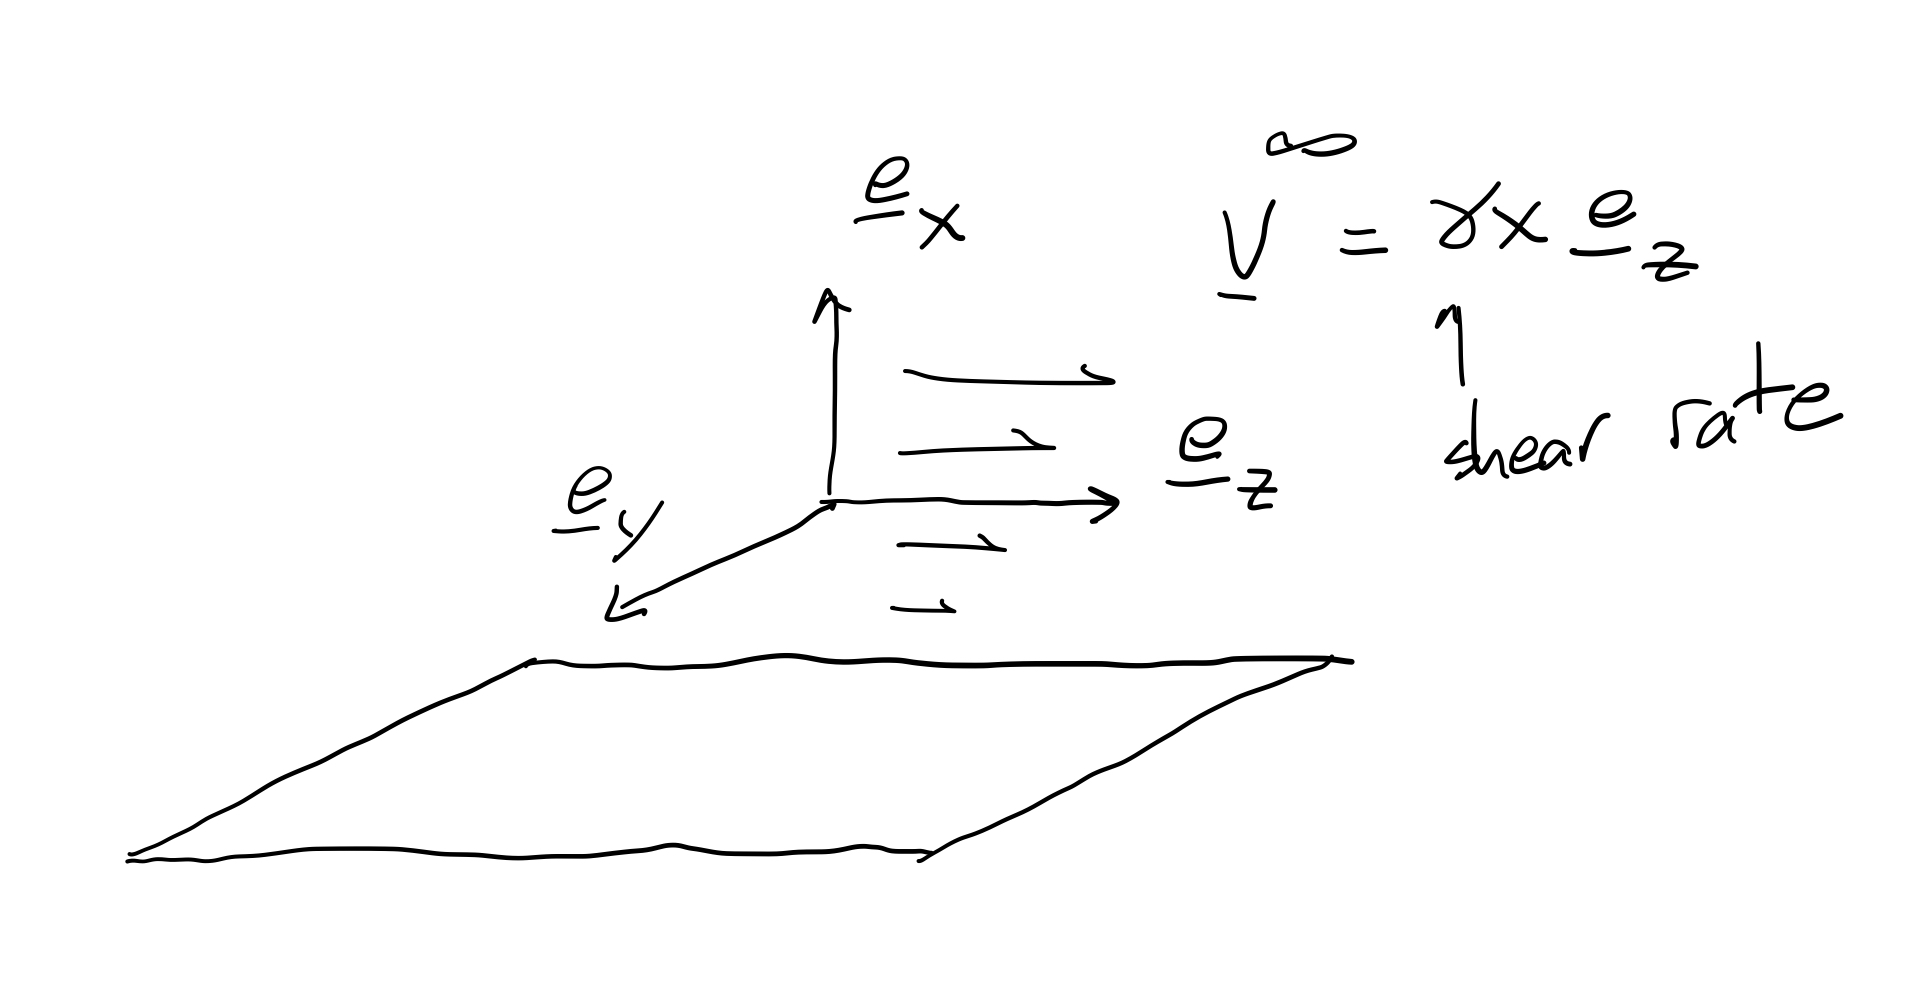
\includegraphics[width=.5\textwidth]{axes}
  \end{center}
\item The mesh is generated on the ellipsoid in the reference
  configuration, where the minor axis $\underline{e}_m$ is equal to
  $\underline{e}_x$:
  \begin{center}
    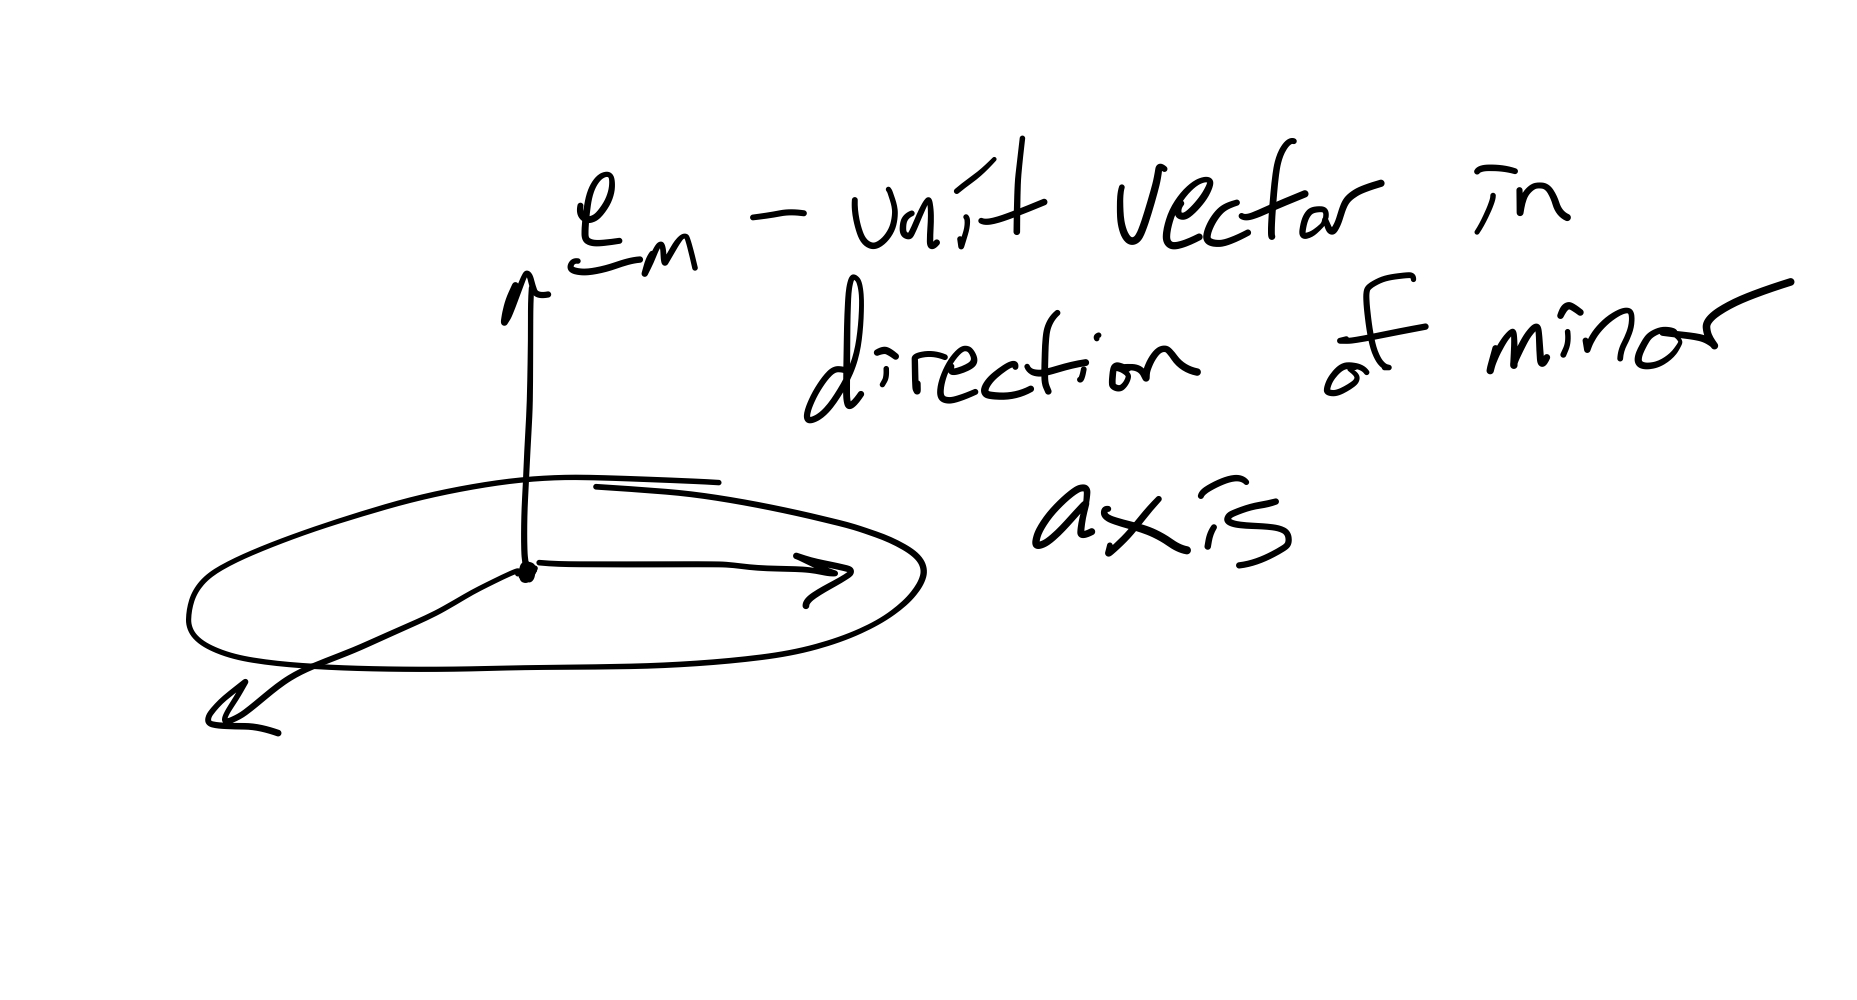
\includegraphics[width=.3\textwidth]{reference}
  \end{center}
\item Any orientation of the ellipsoid can be described by the
  direction of the minor axis $\underline{e}_m$. Because
  $\underline{e}_m$ is a length 3 vector with a fixed length, there
  are two degrees of freedom in the orientation. I decided to use
  spherical coordinates to define the orientation of $\underline{e}_m$
  ($\|\underline{e}_m\| = 1$, so you can think of $\underline{e}_m$ as
  defining a point on the unit sphere). So $\phi$ is the polar angle
  of $\underline{e}_m$ and $\theta$ is the azimuthal angle:
  \begin{center}
    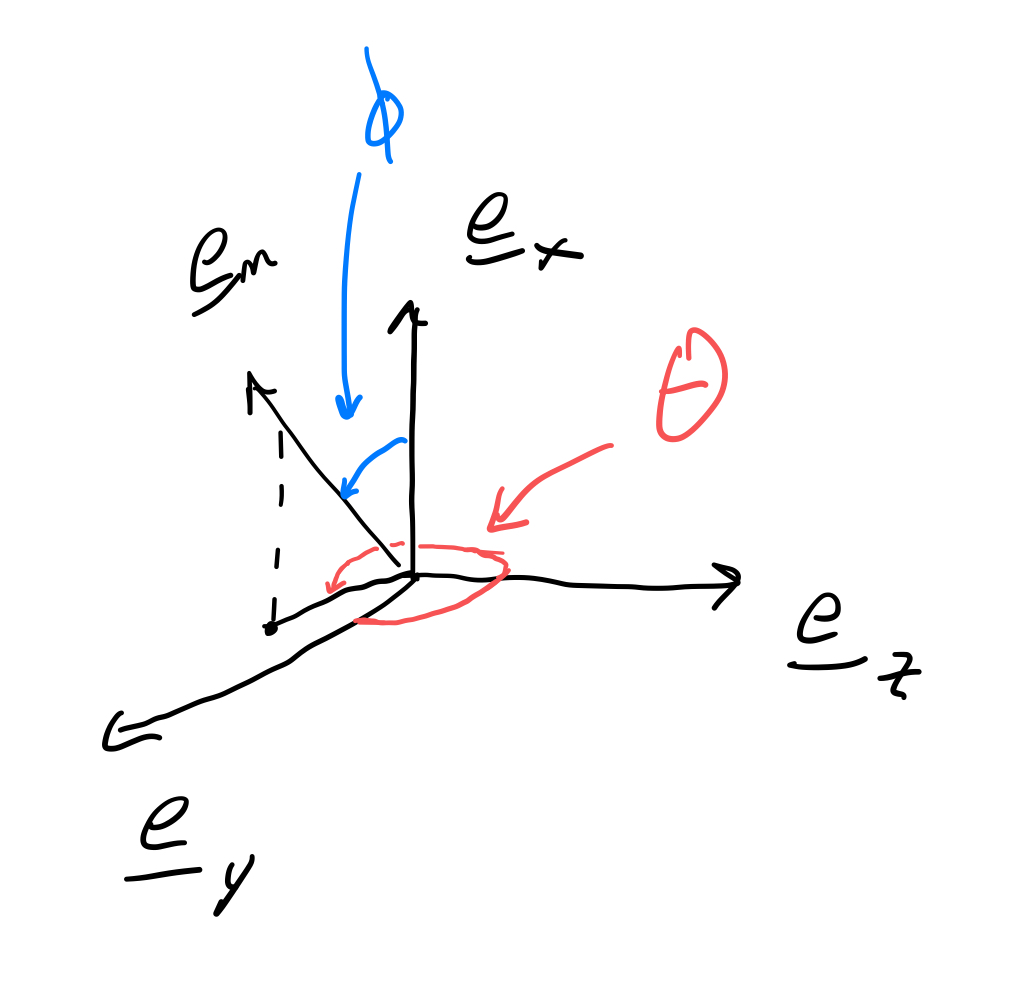
\includegraphics[width=.4\textwidth]{orientation}
  \end{center}
\item Once I generate the mesh on the reference configuration, I
  multiply each point by the rotation matrix:
  \[
    \mathcal{R} =
    \begin{pmatrix}
      \cos\phi & -\sin\phi & 0 \\
      \cos\theta \sin\phi & \cos\theta \cos\phi & -\sin\theta \\
      \sin\theta \sin\phi & \sin\theta \cos\phi & \cos\theta
    \end{pmatrix}
  \]
  which can be decomposed into a simple rotation around the $z$-axis,
  and then a simple rotation around the $x$-axis.

  \[
    \mathcal{R} = R_x(\theta) R_z(\phi) =
    \begin{pmatrix}
      1 & 0 & 0 \\
      0 & \cos\theta & -\sin\theta \\
      0 & \sin\theta & \cos\theta
    \end{pmatrix}
    \begin{pmatrix}
      \cos\phi & -\sin\phi & 0 \\
      \sin\phi & \cos\phi & 0 \\
      0 & 0 & 1
    \end{pmatrix}
  \]
\end{itemize}

\textbf{Convergence experiments}

\begin{itemize}
\item Motivated by Ainley et. al., we want to define the blob
  parameter based on the number of nodes in the mesh. They suggest a
  form: $\epsilon = C h^m$, where $h$ is a characteristic distance
  between adjacent nodes. On a sphere, $h$ is defined as $h =
  \sqrt{4\pi a^2 / N}$ where $N$ is the number of nodes. It seems like
  the natural extension of this to the ellipsoid is $h = \sqrt{S / N}$
  where $S(a, b)$ is the surface area of the ellipsoid with a major
  axis of length $a$ and minor axis of length $b$.
\item In their experiments, they choose the parameters $C$ and $n$
  based on ``reasonable computational results,'' but they don't
  elaborate further.
\item So I ran a series of computational experiments for a range of
  $C$ and $n$ values, with $N$ from 98 to 7,778 nodes. 
\item At each level, (i.e. for each $N$) I compute the resistance
  matrix $A_N$ of the ellipsoid and the force and torque vector
  $\underline{s}_N$ associated with a linear shear flow with shear
  rate 1.
\item Then I define the absolute error to be
  $\hat{e}_\ell = \max(\max_{i,j} (a_{N_\ell} - a_{N_\tn{max}})_{ij},
  \max_i (\underline{s}_{N_\ell} -
  \underline{s}_{N_\tn{max}})_i)$.
\item To find the relative error, I normalized the absolute error by
  $\max(\max_{i,j} (a_{N_\tn{max}})_{ij}, \max_i
  (\underline{s}_{N_\tn{max}})_i)$
\item Error plots for $C = 0.6, 0.8, 1.0$ and $n = 0.8, 0.9, 1.0$ are
  shown below:
  \begin{center}
    \includegraphics[width=.5\textwidth]{ce_convergence}    
  \end{center}
\item I tested smaller values of $C$, but the resistance matrices
  didn't converge (all the absolute errors were $\sim 10^{-14}$).
\item Apart from the small values of $C$ where there was \emph{no}
  convergence, is isn't clear that any of these choices of $C$ and $n$
  are converging faster than any others. (I also don't know what to
  make of the fact that the estimate of the rate of convergence $p$ is
  different at every level of the convergence test).

  This table shows the results of the convergence test for $C = 0.6$,
  $n = 1.0$, but the others have similar $p$ estimates (up to the 2nd
  decimal place)

  \begin{center}
    \begin{tabular}{cccc}\toprule
      $h$ & $N$ & error & $p \approx \frac{\log(e_{i+1} /
                          e_i)}{\log(h_{i+1} / h_i)}$ \\ \midrule
      0.417402642872 & 98 & 0.167935355611 & 1.34640112441 \\
      0.21031709772 & 386 & 0.0667336108054 & 1.46936156291 \\
      0.140413636287 & 866 & 0.0368572277313 & 1.69685978229 \\
      0.105363469903 & 1538 & 0.0226407930285 & 2.04886389757 \\
      0.0843105128131 & 2402 & 0.0143398475575 & 2.61787193704 \\
      0.0702676999165 & 3458 & 0.00890026254931 & 3.66438428468 \\
      0.0602340785528 & 4706 & 0.00506064836056 & 6.22112211895 \\
      0.0527074438112 & 6146 & 0.00220579802183 &  \\ \bottomrule
    \end{tabular}    
  \end{center}

\item Does this mean any of the $C$ and $n$ values in the tested range
  is reasonable?
\item Next, I ran convergence tests for different distances from the
  wall, and different orientations:

  \begin{center}
    \includegraphics[width=0.5\textwidth]{ho_convergence}
  \end{center}
\item It looks like distance is the most important factor in the error of the
  estimates of the resistance matrix and shear vector; the curves seem
  to be separated into groups by distance, not orientation
\item I generated convergence tables for each distance, in the
  orientation $\theta = \phi = 0$; most of them looked similar to the
  table above, but the shortest distance had higher rates of
  convergence at the coarsest grid sizes:

  \begin{center}
    \begin{tabular}{cccc} \toprule
      $h$ & $N$ & error & $p \approx \frac{\log(e_{i+1} /
                          e_i)}{\log(h_{i+1} / h_i)}$ \\ \midrule
      0.417402642872 & 98 & 1.34833689201 & 2.77134081757 \\
      0.21031709772 & 386 & 0.201754848315 & 2.31607646384 \\
      0.140413636287 & 866 & 0.079146723919 & 2.37078783949 \\
      0.105363469903 & 1538 & 0.0400636145436 & 2.53348335535 \\
      0.0843105128131 & 2402 & 0.02277654397 & 2.96828866318 \\
      0.0702676999165 & 3458 & 0.0132623058337 & 3.94979443053 \\
      0.0602340785528 & 4706 & 0.00721646649492 & 6.48655552995 \\
      0.0527074438112 & 6146 & 0.00303596613079 &  \\ \bottomrule
    \end{tabular}
  \end{center}
\item One choice I made in the above experiments was to only test
  distances $> 1.5$, so that no matter what the orientation is, the
  ellipsoid cannot intersect the wall
\item So I ran another set of experiments with the orientation of the
  ellipsoid fixed to the reference configuration, and varied the
  distance of the wall between 1.5 and 0.501:

  \begin{center}
    \includegraphics[width=.5\textwidth]{dist_convergence}
  \end{center}
\item As expected, as the platelet gets closer to the wall the
  estimates get worse more quickly as the mesh coarsens (except for
  the $d = 0.6$ test. Why?).
\item Like in the previous sets of experiments, the estimated
  convergence rate was higher for experiments with a smaller distance.

  For one example, here is the table for $d = 0.51$:
  \begin{center}
    \begin{tabular}{cccc} \toprule
      $h$ & $N$ & error & $p \approx \frac{\log(e_{i+1} /
                          e_i)}{\log(h_{i+1} / h_i)}$ \\ \midrule
      0.417402642872 & 98 & 410.726776849 & 4.3784453677 \\
      0.21031709772 & 386 & 20.425594675 & 3.26143273447 \\
      0.140413636287 & 866 & 5.46898153398 & 3.0992129362 \\
      0.105363469903 & 1538 & 2.24582044745 & 3.36699817335 \\
      0.0843105128131 & 2402 & 1.06028239045 & 3.90587416521 \\
      0.0702676999165 & 3458 & 0.52043365923 & 4.94563886231 \\
      0.0602340785528 & 4706 & 0.242904485374 & 7.51685489364 \\
      0.0527074438112 & 6146 & 0.0890596690237 &  \\ \bottomrule
    \end{tabular}
  \end{center}
\end{itemize}

\textbf{Next}
\begin{itemize}
\item I want to go to finer grid meshes for small distances in order
  to better resolve the errors for those
\item Parallelize the generation of the linear system to find
  stokeslet strengths (accounts for a significant proportion of the
  total computation time)
\item Try a couple of different orientations for the small distances
  and just exclude cases where a node is outside the domain
\item Find the equations of motion for the ellipsoid ($d$ is easy,
  $\theta$ and $\phi$ require a bit of thought)
\end{itemize}


% \large{\textbf{Jump-Velocity Model}}

% \begin{figure}[h]
%   \centering
%   \schemestart
%   $U$ \arrow(u1--vv){<=>[$k_\tn{on}$][$k_\tn{off}$]} $V$
%   \arrow(@u1--ff){<=>[*{0}$k_\tn{on}^F$][*{0}$k_\tn{off}^F$]}[-90] $F$
%   \arrow(--vf){<=>[$k_\tn{on}$][$k_\tn{off}$]} $VF$
%   \arrow(@vv--@vf){<=>[*{0}$k_\tn{on}^F$][*{0}$k_\tn{off}^F$]}
%   \arrow(@u1--ww){->[*{0}$k_\tn{escape}$]}[90]
%   \arrow(@vv--vw){->[*{0}$k_\tn{escape}$]}[90]
%   \schemestop
%   \caption{Jump velocity model with escape}
%   \label{fig:escape-diagram}
% \end{figure}

% \begin{itemize}
% \item One prediction from the jump-velocity model with escape is that
%   the number of dwells in a trajectory should be geometrically
%   distributed. Basically, the probability that a platelet re-binds
%   after unbinding is $a = \frac{k_\tn{on}}{k_\tn{on} + k_\tn{escape}}$,
%   and so the number of binding events that occur before the platelet
%   escapes is a geometric distribution ($p(n) = (1 - a) a^{n-1}$).
% \item A platelet that is not bound to the surface has two possible
%   fates: it can either re-bind with probability $a$ (in which case it
%   must unbind at some point again and return to the same state), or it
%   can escape with probability $1 - a$.
%   \begin{center}
%     \includegraphics[width=.3\textwidth]{step-escape.png}
%   \end{center}
% \item Therefore we can estimate $a$ with the mean number of dwells a
%   platelet takes before escaping: $\mu_\tn{dwell num.} = (1 -
%   a)^{-1}$. Figure \ref{fig:ndwells} shows the number of dwells per
%   trajectory in the two whole blood experiments.
  
%   \begin{figure}[h]
%     \centering
%     \includegraphics[width=\textwidth]{num_dwells}
%     \caption{Number of dwells per trajectory in experiments and
%       predicted by a geometric distribution.}
%     \label{fig:ndwells}
%   \end{figure}
% \item We need another estimate to uniquely find $k_\tn{on}$ and
%   $k_\tn{escape}$.
% \item It turns out the distribution of step times is an exponential
%   distribution with rate $k_\tn{tot} = k_\tn{on} + k_\tn{escape}$, and
%   so we can estimate $k_\tn{tot}$ with the average step time:
%   $\mu_\tn{step time} = 1 / k_\tn{tot} = 1 / (k_\tn{on} +
%   k_\tn{escape})$. With these estimates for $k_\tn{on}$ and
%   $k_\tn{escape}$ (along with the dwell time estimate for
%   $k_\tn{off}$), we get the following estimates for the primed and
%   unprimed experiments:
%   \begin{table}[h]
%     \centering
%     \begin{tabular}{rccc} \toprule
%       & $k_\tn{on}$ & $k_\tn{escape}$ & $k_\tn{off}$ \\ \midrule
%       FFW & $5.24 \pm 1.25$ & $2.42 \pm 0.58$ & $0.16 \pm 0.03$ \\
%       HFW & $0.13 \pm 0.12$ & $0.48 \pm 0.47$ & $0.14 \pm 0.06$ \\
%       \bottomrule 
%     \end{tabular}
%     \caption{Table of parameter estimates for the unprimed and primed
%       experiments}
%     \label{tab:par-est}
%   \end{table}
  
%   Based on these estimates, the on rate increases in the primed
%   experiment while the off rate remains unchanged. For the escape
%   rates, we get the (maybe) counter-intuitive result that the escape
%   rate increases in the priming experiment. I don't have an
%   explanation for this; I'll have to do some more thinking about it
%   first. 
% \item Figure \ref{fig:fbg-whl-step} shows the
%   distribution of step times in simulations and experiments, and there
%   is good agreement for both primed and unprimed platelets.

%   \begin{figure}[h]
%     \centering
%     \includegraphics[width=\textwidth]{fbg_whl_step}
%     \caption{Distribution of step times in experiments and in
%       simulations}
%     \label{fig:fbg-whl-step}
%   \end{figure}
% \item There is also good agreement in the escape time (or moving time)
%   between simulations and experiments (Figure \ref{fig:fbg-whl-esc})
%   and the trajectories look qualitatively similar (Figure
%   \ref{fig:fbg-whl-traj-sim}) 

%   \begin{figure}[h]
%     \centering
%     \includegraphics[width=\textwidth]{fbg_whl_esc}
%     \caption{Escape time distributions in experiments (solid lines)
%       and simulations (dashed lines)}
%     \label{fig:fbg-whl-esc}
%   \end{figure}

%   \begin{figure}[h]
%     \centering
%     \includegraphics[width=\textwidth]{fbg_whl_traj_sim}
%     \caption{Experimental and simulated platelet trajectories}
%     \label{fig:fbg-whl-traj-sim}
%   \end{figure}
% \item The distribution of average velocities is still not capturing
%   the long tail on the average velocity distribution (Figure
%   \ref{fig:fbg-whl-vel}) 

%   \begin{figure}[h]
%     \centering
%     \includegraphics[width=\textwidth]{fbg_whl_vel}
%     \caption{Distribution of time-averaged velocities in experiments
%       (solid line) and simulations (dashed line)}
%     \label{fig:fbg-whl-vel}
%   \end{figure}
% % \item Still to do:
% %   \begin{itemize}
% %   \item Figure out if it is tractable to write a distribution of
% %     effective platelet off rates as a function of individual receptor
% %     on/off rates.
% %   \end{itemize}

% \end{itemize}

% \begin{figure}[h]
%   \centering
%   \schemestart
%   $U$ \arrow(u1--vv){<=>[$k_\tn{on}$][$k_\tn{off}$]} $V$
%   \arrow(@u1--ff){<=>[*{0}$k_\tn{on}^F$][*{0}$k_\tn{off}^F$]}[-90] $F$
%   \arrow(--vf){<=>[$k_\tn{on}$][$k_\tn{off}$]} $VF$
%   \arrow(@vv--@vf){<=>[*{0}$k_\tn{on}^F$][*{0}$k_\tn{off}^F$]}
%   \schemestop
%   \label{fig:primed-states}
% \end{figure}

% \begin{itemize}
% \item Last time: step times in simulations only converge to the
%   fit distribution of step times when the length $L$ of the simulation
%   domain is long. Running simulations through a shorter domain biases
%   the simulated distribution of step times to be smaller than expected.
% \item Figure \ref{fig:step-time}---Figure \ref{fig:traj-plots-200} show step
%   time distributions and trajectories from simulations run through
%   domains of various lengths, as well as simulated step time
%   distributions when only looking at trajectories in a $2.5 \, \mu m$
%   window. Restricting the ``viewing window'' in the longer
%   stochastic experiments seems equivalent (and I suspect is) to
%   running the simulations through a short domain.
% \item I think that estimating the effective platelet on rate as the
%   inverse of the mean step time \emph{overestimates} the effective on
%   rate. In our experiments, longer steps are more likely to get cut
%   off (and therefore not counted) because platelets are more likely to
%   leave the domain on a long step. Are longer steps more likely to get
%   cut off in observed trajectories? If they are, then our estimate of
%   effective on-rate is an over-estimate of the true effective on rate.
% \item I also imported Emma's data, and it is plotted in Figure
%   \ref{fig:emma-data}. Platelets are moving much faster in these
%   experiments than in their previous experiments. I plotted the new
%   trajectories alongside the whole blood trajectories, but they didn't
%   mention whether these experiments were done with whole blood or
%   PRP. In either case, the new trajectories have higher velocities
%   than the old trajectories. I've asked them whether these are whole
%   blood or PRP trajectories, and what the shear rate on these
%   experiments are (the old ones are at 100/s wall shear rate.)
% \item We may be able to draw a stronger connection back to
%   mechanism. Qi et. al., 2019, quote a result connecting effective
%   platelet on and off rates back to receptor on/off rates, although
%   they don't give any details on how they use that relation.
% \end{itemize}

% \begin{figure}
%   \centering
%   \includegraphics[width=\textwidth]{fbg_step_sim}
%   \caption{Step time distributions with $L = 2.5 \, \mu m$}
%   \label{fig:step-time}
% \end{figure}

% \begin{figure}
%   \centering
%   \includegraphics[width=\textwidth]{fbg_step_sim_window}
%   \caption{Step time distributions in a $L = 2.5 \, \mu m$ window}
%   \label{fig:step-time-window}
% \end{figure}

% \begin{figure}
%   \centering
%   \includegraphics[width=\textwidth]{fbg_step_long}
%   \caption{Step time distributions with $L = 50 \, \mu m$.}
%   \label{fig:step-time-long}
% \end{figure}

% \begin{figure}
%   \centering
%   \includegraphics[width=\textwidth]{fbg_step_sim_100}
%   \caption{Step time distributions with $L = 100 \, \mu m$}
%   \label{fig:step-time-100}
% \end{figure}

% \begin{figure}
%   \centering
%   \includegraphics[width=\textwidth]{fbg_step_sim_200}
%   \caption{Step time distributions with $L = 200 \, \mu m$.}
%   \label{fig:step-time-200}
% \end{figure}

% \begin{figure}
%   \centering
%   \begin{subfigure}{\textwidth}
%     \includegraphics[width=\textwidth]{fbg_prp_traj_sim}
%     \caption{Observed (left) and simulated (right) (with $L=2.5 \, \mu m$)
%       trajectories in PRP.}
%   \end{subfigure}
%   \\
%   \begin{subfigure}{\textwidth}
%     \includegraphics[width=\textwidth]{fbg_whl_traj_sim}
%     \caption{Observed (left) and simulated (right) (with $L=2.5 \, \mu m$)
%       trajectories in whole blood.}
%   \end{subfigure}
%   \caption{Trajectories of primed (red) vs unprimed (blue) platelets
%     in experiments and simulations.}
%   \label{fig:traj-plots}
% \end{figure}

% \begin{figure}
%   \centering
%   \begin{subfigure}{\textwidth}
%     \includegraphics[width=\textwidth]{fbg_prp_traj_sim_window}
%     \caption{Observed (left) and simulated (right) (in a
%       $L=2.5 \, \mu m$ window) trajectories in PRP.}
%   \end{subfigure}
%   \\
%   \begin{subfigure}{\textwidth}
%     \includegraphics[width=\textwidth]{fbg_whl_traj_sim_window}
%     \caption{Observed (left) and simulated (right) (in a
%       $L=2.5 \, \mu m$ window) trajectories in whole blood.}
%   \end{subfigure}
%   \caption{Trajectories of primed (red) vs unprimed (blue) platelets
%     in experiments and simulations.}
%   \label{fig:traj-plots-window}
% \end{figure}

% \begin{figure}
%   \centering
%   \begin{subfigure}{\textwidth}
%     \includegraphics[width=\textwidth]{fbg_prp_traj_sim_long}
%     \caption{Observed (left) and simulated (right) (with $L=50 \, \mu m$)
%       trajectories in PRP.}
%   \end{subfigure}
%   \\
%   \begin{subfigure}{\textwidth}
%     \includegraphics[width=\textwidth]{fbg_whl_traj_sim_long}
%     \caption{Observed (left) and simulated (right) (with $L=50 \, \mu m$)
%       trajectories in whole blood.}
%   \end{subfigure}
%   \caption{Trajectories of primed (red) vs unprimed (blue) platelets
%     in experiments and simulations.}
%   \label{fig:traj-plots-long}
% \end{figure}

% \begin{figure}
%   \centering
%   \begin{subfigure}{\textwidth}
%     \includegraphics[width=\textwidth]{fbg_prp_traj_sim_100}
%     \caption{Observed (left) and simulated (right) (with $L=100 \, \mu m$)
%       trajectories in PRP.}
%   \end{subfigure}
%   \\
%   \begin{subfigure}{\textwidth}
%     \includegraphics[width=\textwidth]{fbg_whl_traj_sim_100}
%     \caption{Observed (left) and simulated (right) (with $L=100 \, \mu m$)
%       trajectories in whole blood.}
%   \end{subfigure}
%   \caption{Trajectories of primed (red) vs unprimed (blue) platelets
%     in experiments and simulations.}
%   \label{fig:traj-plots-100}
% \end{figure}

% \begin{figure}
%   \centering
%   \begin{subfigure}{\textwidth}
%     \includegraphics[width=\textwidth]{fbg_prp_traj_sim_200}
%     \caption{Observed (left) and simulated (right) (with $L=200 \, \mu m$)
%       trajectories in PRP.}
%   \end{subfigure}
%   \\
%   \begin{subfigure}{\textwidth}
%     \includegraphics[width=\textwidth]{fbg_whl_traj_sim_200}
%     \caption{Observed (left) and simulated (right) (with $L=200 \, \mu m$)
%       trajectories in whole blood.}
%   \end{subfigure}
%   \caption{Trajectories of primed (red) vs unprimed (blue) platelets
%     in experiments and simulations.}
%   \label{fig:traj-plots-200}
% \end{figure}

% \begin{figure}
%   \centering
%   \includegraphics[width=\textwidth]{emma_data_traj}
%   \caption{Trajectory plots of Emma's data (plotted in magenta
%     (primed) and cyan (unprimed)), along with the previous
%     fibrinogen whole blood trajectories}
%   \label{fig:emma-data}
% \end{figure}

\bibliographystyle{plain}
\bibliography{/Users/andrewwork/Documents/grad-school/thesis/library}

\end{document}




